\documentclass[10pt,conference,compsocconf]{IEEEtran}
\usepackage[T1]{fontenc}
\usepackage[utf8]{inputenc}
\usepackage{url}
\usepackage{comment}
\usepackage{graphicx}
\usepackage{multirow}
\usepackage{booktabs}
\usepackage{amsmath}

\usepackage{tikz}
\usetikzlibrary{fit}

\usepackage{acronym}
\acrodef{iaas}[IaaS]{Infrastructure as a Service}
\acrodef{SaaS}{Software as a Service}
\acrodef{PaaS}{Platform as a Service}
\acrodef{dag}[DAG]{directed acyclic graph}
\acrodef{vm}[VM]{Virtual Machine}
\acrodef{pm}[PM]{Physical Machine}
\acrodef{btu}[BTU]{billing time unit}
\acrodef{EC2CU}{EC2 Compute Unit}
\acrodef{HPC}{High Performance Computing}
\acrodef{unistra}{University of Strasbourg}
\acrodef{rv}[RV]{random variable}
\acrodef{pdf}[PDF]{probability density function}
\acrodef{cdf}[CDF]{cumulative distribution function}
\acrodef{mcs}[MCS]{Monte-Carlo simulation}
\acrodefplural{mcs}[MCS's]{Monte-Carlo simulations}
\acrodef{des}[DES]{discrete event simulation}
\acrodef{ci}[CI]{confidence interval}

\newcommand*\rot{\rotatebox{90}}
\newcommand{\pmpc}[1]{$\pm#1\%$}
\newcommand{\etal}[1]{\emph{#1 et al.}}
\newcommand{\pc}[1]{$#1\%$}

%\IEEEtriggeratref{15}

%\title{Modeling the accuracy of Monte-Carlo approach for Cloud based workflow
%  simulations.}

\title{Executing Batch Jobs on Clouds: How to Predict Reality Accurately?}


\author{\IEEEauthorblockN{Luke~Bertot 
			and Stéphane~Genaud 
			and Julien~Gossa}
	\IEEEauthorblockA{Icube-ICPS --- UMR 7357, Univeristé de Strasbourg, CNRS\\
		P\^ole API Blvd S. Bant, 67400 Illkirch\\
		email: \url{lbertot@unistra.fr}, \url{genaud@unistra.fr}, \url{gossa@unistra.fr}}
	}



\begin{document}

\maketitle

\begin{abstract}
  In the  cloud computing  model, cloud providers  invoice clients  for resource
  consumption. Hence, tools helping the client to budget the cost of running his
  application are  of pre-eminent  importance. To  that end,  a number  of cloud
  simulators have been  proposed by researchers. However, the  attempts to reach
  reliable  predictions are  hampered by  the opacity  regarding the  underlying
  hardware platform, and by the  multi-tenant nature of clouds. Those make job
  runtimes both  variable and hard to  predict.  In this paper,  we investigate
  which parameters are the most  influential in the
  prediction of the actual execution behavior in terms of cost and total runtime,
  through two real  use-cases.

  We consider the execution  of batch jobs on an  actual platform, one example
  being a  bag-of-tasks and the other  one a workflow, whose  jobs are scheduled
  using typical  heuristics based on  the user  estimates of job  runtimes.  We
  propose an  improved simulation framework  based on the Monte-Carlo  method to
  study the  relationship between the  precision of  the user estimates  and the
  accuracy of the simulation results regarding  cost and makespan. Based on this
  stochastic process,  predictions are expressed as  interval-based makespan and
  cost.   We show  that, most  of the time, imprecisions  in  user estimates are
  largely amortized in the final predictions but still can capture real
  observations. Finally, we identify evidence of the influence of the scheduling 
  heuristics on the accuracy of the method.
  % JG : je ne comprends pas le `` but still can capture real observations''
\end{abstract}

\begin{IEEEkeywords}
cloud computing, computer simulation, monte carlo methods.
\end{IEEEkeywords}

%\tableofcontents

\section{Introduction.}


Over the  last decade, the advancement  of virtualization techniques has  led to
the emergence of new economic  and exploitation approaches of computer resources
in  \ac{iaas},  one form  of cloud  computing. In  this model,  all
computing resources  are made available  on demand by third-party  operators and
paid based  on usage.  The  ability to provision  resources on demand  is mainly
used in two ways.  Firstly, it can serve for scaling purposes where new machines
are  brought online  to  fulfill  service availability  in  the  face of higher 
workloads.  This approach  is used  for  providing services  and allows  for a  lower
baseline  cost  while  still  being  able  to deal  with  spikes  in  demand  by
provisioning machines on the fly. Secondly, it is useful for parallelizing tasks
to achieve a shorter makespan (i.e.\ the time between the submission of the first
task and the completion of the  last task)  at equal  cost, this  approach being  often used  for
scientific  and  industrial  workloads  when runtime  is  heavily  dependent  on
computing power.  This  approach is made possible by the  pricing model of cloud
infrastructures, as  popularized by AWS\footnote{Amazon Web  Services}, in which
payment  for computing  power, provided  as \acp{vm},  happens in  increments of
arbitrary lengths  of time, \ac{btu}, usually  of one hour. Running  two \acp{vm}
side by side for one \acp{btu} actually costs the same as running one \ac{vm} for two
\acp{btu}, but every \ac{btu} started is owed in full.

This model  offers the client  an almost complete freedom  to start or  stop new
servers as long as the price can be afforded. However, for parallel applications composed
of a set of jobs, it  quickly  becomes  difficult  to manually  provision  the
resources in an  efficient way.  The use of a  scheduler becomes unavoidable for
such workloads.   In this paper, we  are interested in predicting  the execution
time  and cost  of such  workloads, in  which the  scheduling plays  an
important role.  In  this study, we consider two  opposite scheduling strategies
to put forward their impact on execution behavior.
%--[We will review in the related work section several other scheduling approaches.]


%----------------------- prediction tools --------------------------------------
Independently of  scheduling decisions, the accurate prediction  of the  runtime of
complex workloads is hampered by  multiple factors.  First \ac{iaas} operates in
an opaque  fashion~: the exact nature  of the underlying platforms  is unknown,
and their hardware are subject to evolution as operators update their data-centers
over  the years  with new  servers and  equipment.  Secondly  cloud systems  are
multi-tenant by nature. This adds uncertainty due to contention  on network and
memory accesses, depending on how \acp{vm} are scheduled and the activity of your
\emph{neighbors}.   Even   when  \ac{iaas}  operators  attempt   to  mask  these
irregularities in computing  power and network access by  guaranteeing a minimum
performance, variability occurs ini the presence of \emph{less-than-noisy-neighbors}
as it is not in the interest of the \ac{iaas} operators to limit power available
over the guaranteed minimums.  These factors  increase the difficulty
of  modeling   job  execution  times, which is already difficult enough,  as  shown
in~\cite{Lastovetsky05}.

In this regard,  the prediction is highly dependent on  the underlying simulator
of the system and on the phenomena it  can capture. In this work, we rely on the
SimGrid~\cite{simgrid}  simulation toolkit, enabling us to build discrete event
simulators of distributed systems such as Grids, Clouds, or HPC systems. SimGrid
has   been    chosen   for    its   well-studied   accuracy    against   reality
(e.g.~\cite{StanisicTLVM15,VelhoSCL13}).    In   particular,  given   a   precise
description  of the  hardware platform,  its  network model  takes into  account
network contention in presence of multiple communication flows.

However, we may not be able to provide a fully accurate platform description, or
be unable  to estimate  the network  cross-traffic, yielding  a distorsion  between
simulation and reality.  To deal with this problem, the  standard approach is to
consider job runtimes to  be stochastic.  Every job can be  modeled by a \ac{rv}
that models the whole spectrum of possible runtimes. These \acp{rv} are the basis
required for a stochastic simulation.  Such simulations output a random variable
of the  observed phenomenon (\emph{makespan}  or \emph{\ac{btu}}) which  in turn
can  be  used to  create  intervals  of  possible  results with  their  assorted
confidence.

In this paper, we propose a stochastic method to enrich the classical prediction
based  on the  discrete-event simulator  SimGrid,  and we  study the  conditions
needed for  this approach to be  relevant. This study  is carried out in  a real
setting,  described in  section~\ref{sec:work-context},  where the  applications
use-cases, the scheduler, and the  experimental observations are presented.  The
stochastic     framework     we     propose     is     then     presented     in
section~\ref{sec:enriched-sim}  and is  evaluated in  section~\ref{sec:eval}. We
finally conclude by  discussing in section~\ref{sec:disc} the possible
improvements and the  limits of the approach.


\section{Related Work}
\begin{comment}
\begin{table*}
	\centering
	\caption{Comparison of capabilities and functions of 5 common cloud
	simulators}
	\label{tab:simcmp}
\begin{tabular}{|c||c|c|c||c|c|c|c|}
	\hline
	%% line 1
	& \multicolumn{3}{c||}{Application} &
	\multicolumn{2}{c|}{CPU}&Network&Disk\\
	\cline{2-8}
	%%line 2
	Simulator &trace%(a) 
                  &model%(b)
                  &code%(c)
                  &timed%(d)
                  &\#instr%(e)
		  &type 
		  &max precision\\
	\hline
	%%line 3
	CloudSim\cite{cloudsim} & & & \bf X &&\bf
	X&store\&forward&seek+transfert\\ \hline
	ICanCloud\cite{icancloud} & & & \bf X &&\bf X&packet& bloc \\ \hline
	GroudSim\cite{groudsim} & & & \bf X &&\bf X&flow& n/a\\\hline
	GreenCloud\cite{greencloud} & & \bf X &&&\bf X&packet& n/a\\ \hline
	SimGrid\cite{simgrid}& \bf X & \bf X & \bf X &\bf X&\bf X& flow/packet &
	seek+transfert \\
	\hline
\end{tabular}
\end{table*}
\end{comment}


\subsection{Simulation}

Because they allow for experiments on functionality without having to build a
dedicated platform, simulations are a cornerstone of the study of distributed
systems and clouds.  
%JG : ``on fucntionality'' me parait ambigue.

Most cloud  simulators are based on  \ac{des}. In \aclp{des} the  simulation is a
serie of events changing the state of  the simulated system.  For instance, events can be the
start  (or  end)  of  computations or of communications.
The simulator will jump from one event to the next,
updating the  times of  upcoming events to  reflect the change  of state  in the
simulation.   Such  \ac{des}  based  simulators  require  at  least  a  platform
specification  and  an  application  description.   The  platform  specification
describes both the physical nature of the cloud, e.g.~machines and networks, and
the management rules, e.g.~\ac{vm} placement and availability.  Depending on the
simulator,  platform  specification  can  be  done  through  user  code,  as  in
CloudSim~\cite{cloudsim} for example, or  through platform description files, as
is  mostly  the case  in  SimGrid~\cite{simgrid}.   The application  description
consists in  a set of  computing and communicating  tasks, often described  as an
amount of computation and communication  to perform. The simulator computes
their duration based on the platform  specification, and its CPU and network models.
An  alternative  approach is  to  extrapolate  the  task durations  from  actual
execution traces observed in real executions.
%JG : je ne vois pas l'intérêt de cette dernière phrase.

Available cloud \acp{des} include CloudSim~\cite{cloudsim} a extensible
simulator written in Java, Simgrid~\cite{simgrid} when use in conjunction with
the SCHIaaS cloud interface, the NS2-based GreenCloud~\cite{greencloud} centered
on energy consumption of cloud's network apparatus, the commercial solution
MDCSim~\cite{MDCSim} from Pennsylvania State University,
ICanCloud~\cite{icancloud} which can be run in parallel on multiple machines,
and GroudSim~\cite{groudsim} which can simulate both Grids and Clouds.

At the core of DES  is the  solver. The solver considers the  states of  the system
generated by the platform and previous events  to compute the timing of the future
events. Therefore it defines  which is the next event of the simulation. 
In  most cases, simulators  have a  \emph{bottom-up} approach: The
modeling concerns low-level components  (machines, networks, storage devices), 
and from their interactions emerge the high-level  behaviours.
Working  on disjointed low-level  components make it easier  to tune
the precision  of the model to  the wanted accuracy/speed trade-off.

However, when the simulated system is subject to variability, it is difficult
to formally  establish the  validity of simulation  results. Indeed,  given some
definite inputs,  a DES  outputs a  single deterministic  result, while a real
system  will output  slightly different  results at  each repeated  execution.
Hence, in practice  the simulation is informally regarded as
valid if  its results  are ``close'' to  one or some  of the  real observations.
Notice however  that in the  field of grid or  cloud computing, very  few papers
address the issue of the simulation validity.

\subsection{Stochastic Simulation and Monte-Carlo Method}

\label{sc:relwork-stochastic}
For  more   comprehensive  predictions  in  such   variables  environments,  the
simulation must  be \emph{stochastic}.  In stochastic simulations  inputs become
\acfp{rv} representing the  distribution of possible values  for the parameters.
The  result  of one  such  simulation  is  itself  an \ac{rv}  representing  the
distribution  of the  results.  This  approach has  been used  early to  compute
schedules for task graphs (\ac{dag}) with stochastic durations in the context of
PERT networks~\cite{Slyke63}.

%,  and applied in  the recent  years to
%heterogeneous distributed computing environments.  For example in the context of
%grids,  Tang  et al.~\cite{Tang11}  propose  a  modification of  the  well-known
%scheduling heuristic HEFT  to compute a schedule yielding  the shortest makespan
%given randomly variable task durations. 

Similarly in  our context,  an application is modeled  as a  \ac{dag} in
which the vertices represent the tasks  comprising the application, and the edges
the dependencies between those tasks.  Each vertex can then be assigned its respective
\ac{rv}  representing   its  possible  runtimes.    The  result  is   a  \ac{rv}
representing  the possible  duration for  the execution  of the  whole \ac{dag},
called  \emph{makespan}. A  \ac{rv} is  defined by  its \ac{pdf}  and \ac{cdf},
where  the   \ac{cdf}  is  obtain   by  integrating  the  \ac{pdf}.    Works  on
heterogeneous  grids~\cite{Li97} and  PERT  networks~\cite{Ludwig01} show  that
when  tasks runtimes  are  independent, the  makespan of  successive  tasks is  a
convolution product  of the individual  tasks \acp{rv}, while the  makespan of
parallel tasks  joining is the  product of  the tasks respective  \ac{cdf}. However, this
mathematical approach is computationally intensive, while the
tasks \acp{rv} independence can not be guaranteed in most cases.

Moreover this \ac{dag} based approach implies fixed scheduling. 
But cloud platforms allow additional resources provisioning at anytime.
Thus, users are likely to call on dynamic schedulers that adapt the schedule on the fly
depending of the already executed jobs runtimes and the availability of
resources. With a \ac{dag} representation this is akin to adding
and removing edges depending on the runtime of certain vertices. Edges do not
only represent the dependencies, the inherent constraint between the application
jobs, but also the scheduling, the effective constraint imposed on a job queued
after another.
%JP : peut être grandement simplifié/raccourci pour gagner de la place

Instead  of computing  the resulting  \ac{rv}, a  \ac{mcs} samples  the possible
results by testing  multiple \emph{realizations} in a  deterministic fashion.  A
realization is obtained by drawing a runtime that follows their job's respective 
\ac{rv} for  every job in the  application. Since within a realization each job
has now a  defined runtime, each realization can be  simulated using traditional
methods like \ac{des}.  Eventually, given enough realizations, the distribution of
the simulation  results will  tend towards the  distribution of  the equivalent
stochastic  simulation.  Statistical  fitting  techniques can  then  be used  to
characterize this makespan \ac{rv}.

The development  of heterogeneous distributed computing  environments, grids and
now clouds,  has led  researchers to use  this approach in  this field.   In the
context of grids,  where the number of resources is  fixed during one execution,
Tang et  al.~\cite{Tang11} propose a  modification of the  well-known scheduling
heuristic  HEFT to  compute  a  schedule yielding  the  shortest makespan  given
randomly  variable task  durations. Canon~\cite{Canon10}  have used  \ac{mcs} to
evaluate  the robustness  of \ac{dag}  schedules when  task durations  vary, and
similarly, Zheng et  al.~\cite{Zheng13} evaluate the impact  of this variability
on  makespan.  More  recently,  ElasticSim~\cite{Cai17} as  been  proposed as  a
simulator extending  Cloudsim to integrate resource  auto-scaling and stochastic
task  durations. Similarly  to our  work, ElasticSim  computes a  schedule whose
objective  is  to  minimize  rental  cost excepted  that  they  impose  deadline
constraints.  The  study compares the  simulation results regarding  rental cost
and makespan,  when varying the variability  of task duration and  deadline with
arbitrary  values,  for  several  generated workflows.  By  contrast,  our  work
focuses on how the \ac{mcs} method, under some given variability assumptions, 
captures actual observations.
%JG : ``excepted  that  they  impose  deadline constraints`` n'est pas super bien articulé. Et si ce n'est pas utile, autant enlever.


\section{Work Context}
\label{sec:work-context}

The  study conducted  in this  paper  is build  upon an  original comparison  of
experiments  run in  actual environments  and experimental  results obtained  by
simulation.   To strengthen  the validity  of the  comparison, the  experimental
conditions  for  the  real  setup  and  the  simulation  should  share  as  many
commonalities  as   possible~\cite{PucherGWK15}.   We  describe   hereafter  our
experimental setup.  It consists of two  test applications which are  run on one
side, on a real platform with our scheduler Schlouder and on the other side, are
simulated  with   our  simulator  SimSchlouder   based  on  SimGrid.    The  two
environments are sketched side by side on Figure~\ref{fig:rs}.

\subsection{Test Applications}\label{sc:setup}

To  evaluate Schlouder  performance we  carried out  multiple executions  of two
broadly used scientific  applications. The execution traces for  those runs were
collected  in an  archive.  This backlog  of real  executions  is the  benchmark
against which  our simulation  performance will  be evaluated.  The applications
used are:

\begin{itemize}
\item Montage\cite{montage2009},  the Montage Astronomical Image  Mosaic Engine,
  is designed to  splice astronomical images. The structure  of this application
  is a  fork-join type  workflow. This application  is extremely  data intensive
  with a \emph{commuication-to-computation} ratio superior to $90\%$.

\item OMSSA\cite{Geer2004}, the Open Mass-Spectrometry Search Algorithm, is used
  to analyze  mass-spectrometer results.  The application  is parallelized  as a
  bag-of-tasks, \textit{i.e.}  as a  number of  independent parallel  jobs. This
  application        is        computation        intensive        with        a
  \emph{communication-to-computation} ratio under $20\%$.
\end{itemize}

The executions of these applications each composed  of a set of jobs are driven
by the scheduling policy applied. We detail in the next two sections how these
executions are managed in the actual environment and in simulation.  

\subsection{Real Execution Setup}

In the recent years, we have developed  a client-side job broker for IaaS clouds
called  Schlouder~\cite{Michon17}.  This  broker is  able to  submit the  user's
batch jobs, be  it a set of  independent jobs or a workflow.   The broker's main
role is  to schedule the set  of jobs onto a  set of cloud resources,  which the
broker can scale up  or down.
Technically, the broker  connects to the cloud management  system (for instance,
OpenStack) to  instruct how  the infrastructure should  be provisioned  and then
assigns the jobs to the resources using the Slurm job management system.

As  in almost  all batch  scheduler systems,  the job  description includes  its
runtime  estimation by  the  user called  \emph{user estimate}.   In  case of  a
workflow, the job  dependencies are also provided.   Schlouder uses just-in-time
scheduling where jobs are assigned to \acp{vm} as soon as all their dependencies
are satisfied.  We call \emph{strategy} the  heuristic used by Schlouder to make
provisioning and  scheduling decisions.  A  dozen strategies and  their variants
are available to  the user (details can be found  in~\cite{GenaudG11}), of which
we will use two in this  paper.  Strategies provision \acp{vm} and schedule jobs
based  on  the user  estimates  of  the runtime.   Notice  that  the jobs'  real
runtimes, called \emph{effective  runtimes}, may differ from  the estimates, but
this does not change the initial scheduling decision.

The provisioning and scheduling strategies of Schlouder are bi-objective, namely
cost of renting the resources, and makespan of the execution.  In this paper, we
test the two following strategies which favor one objective or the other:
\begin{itemize}
\item ASAP (or \textit{as soon as possible}): schedules the job immediately onto
  an idle VM, or immediately provisions a new  VM to start the job if no idle VM
  is available.  Hence this strategy tries to minimize the makespan of the batch
  job execution.

\item AFAP (or \textit{as full as  possible}): schedules each job in priority to
	an already available resource whenever the remaining time  before a new
	\ac{btu} begins is greater or equal to the job estimated runtime.
	By solving this bin-packing problem, this strategy tends to minimize the
	monetary cost of the batch execution.
\end{itemize}

The left part  of Figure~\ref{fig:rs} presents the outline of  a real execution.
From the  job set description including  user estimates and dependencies,  and a
strategy   Schlouder  computes   the   scheduling   and  resource   provisioning
decisions. It  then communicates its  requests to the cloud's  frontend, denoted
Controller.   Once the  \acp{vm}  are booted  Schlouder sends  each  job to  its
assigned machine.  Schlouder tracks jobs progression, completing the schedule as
dependencies are  resolved, provisioning \acp{vm}  as needed, and  shutting down
unneeded \acp{vm} as their billing cycle close.

\begin{figure}
	\resizebox{0.5\textwidth}{!}{%
		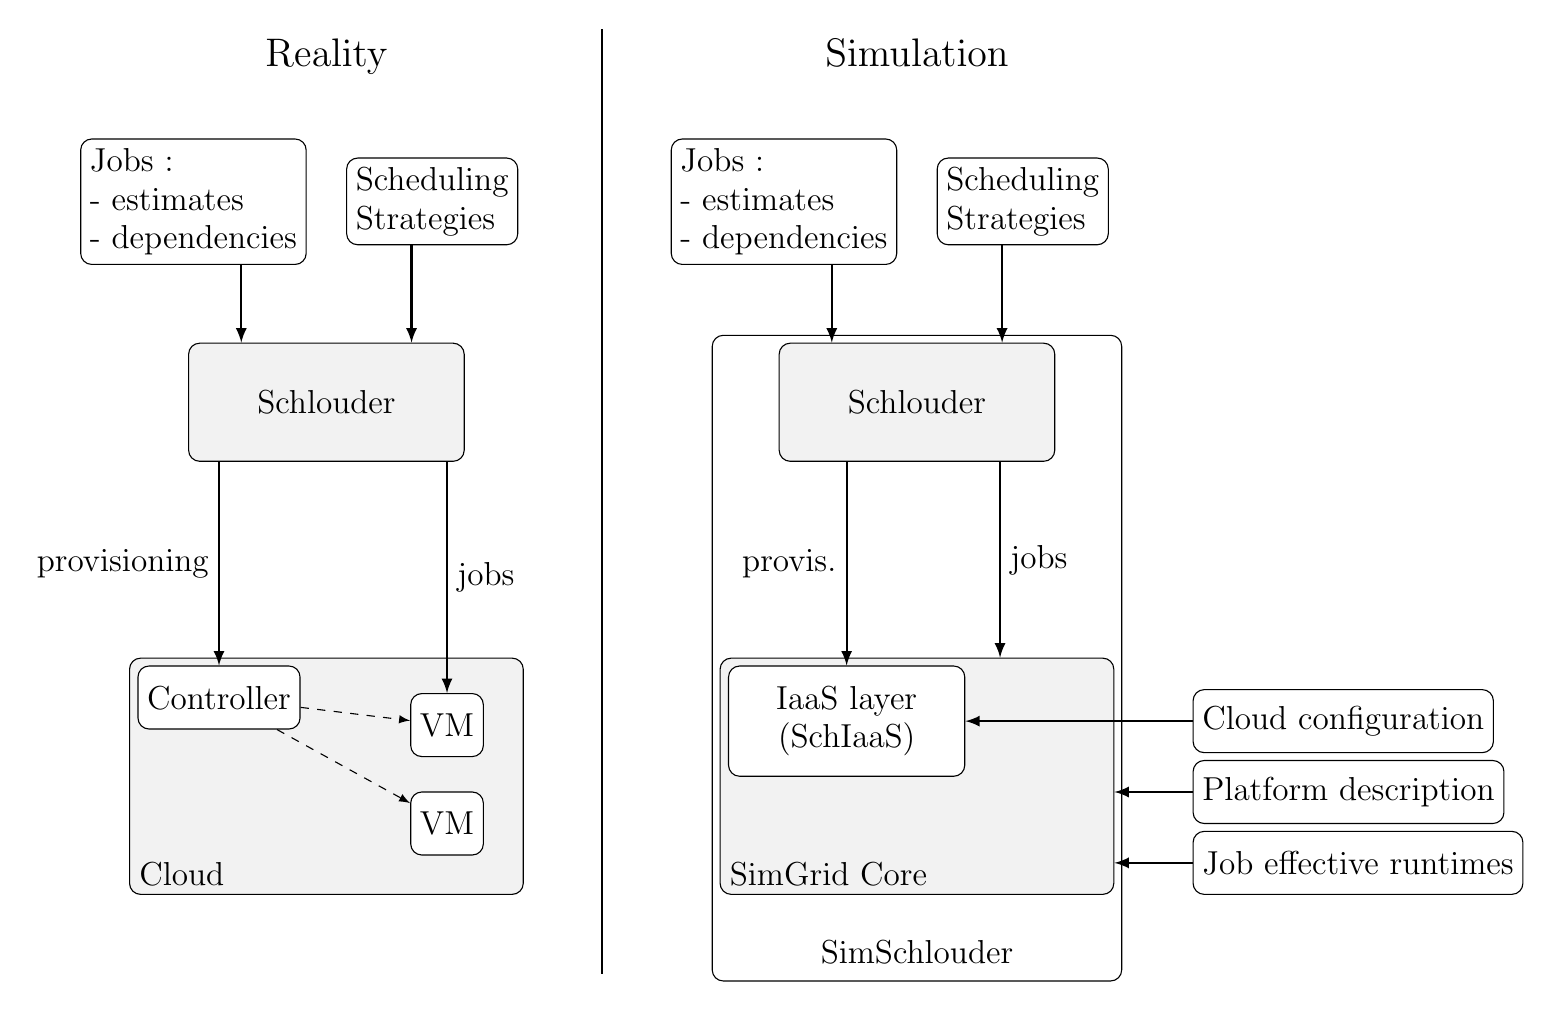
\begin{tikzpicture}[x=1cm,y=1cm,
font=\large,
plate/.style={anchor=south west},
b/.style={
draw,
anchor=south,
minimum width=0.8cm,
minimum height=0.8cm,
rounded corners},
lb/.style={b,anchor=south west},
rb/.style={b,anchor=south east},
fg/.style={fill=gray!10},
fw/.style={fill=white},
]
%Reality
\begin{scope}[shift={(-3.5,0)}]
\node[font=\Large,anchor=north]at(0,11){Reality};
%%Cloud
\node[b,fg,minimum width=5cm,minimum height=3cm]at(0,0){};
\node[plate]at(-2.5,0){Cloud};
\node[rb,fw](vm1)at(2,0.5){VM};
\node[rb,fw](vm2)at(2,1.75){VM};
\node[lb,fw](cc)at(-2.4,2.1){Controller};
\draw[-{latex},dashed](cc)--(vm1);
\draw[-{latex},dashed](cc)--(vm2);
%%Sclouder
\node[b,fg,minimum width=3.5cm,minimum height=1.5cm](schlouder)at(0,5.5){Schlouder};
\draw[-{latex},thick,](schlouder.south-|cc.north)--(cc.north)node[pos=0.5,left]{provisioning};
\draw[-{latex},thick,](schlouder.south-|vm2.north)--(vm2)node[pos=0.5,right]{jobs};
%% Inputs
\node[rb,align=left](jobs)at(-0.25,8){Jobs : \\ - estimates\\ - dependencies};
\node[lb,align=left](conf)at(0.25,8.25){Scheduling\\Strategies};
\draw[-{latex},thick](jobs.south-|schlouder.145)--(schlouder.145);
\draw[-{latex},thick](conf.south-|schlouder.35)--(schlouder.35);
\end{scope}
\draw[thick](0,-1)--(0,11);
%Simulation
\begin{scope}[shift={(4,0)}]
\node[font=\Large,anchor=north]at(0,11){Simulation};
%Simulator
\node[b,minimum width=5.2cm,minimum height=8.2cm]at(0,-1.1){};
\node[anchor=south]at(0,-1){SimSchlouder};
%%Cloud
\node[b,fg,minimum width=5cm,minimum height=3cm](SG)at(0,0){};
\node[plate]at(-2.5,0){SimGrid Core};
\node[lb,fw,minimum width=3cm,minimum height=1.4cm,align=center](cc)at(-2.4,1.5){IaaS layer\\(SchIaaS)};
%%SimSclouder
\node[b,fg,minimum width=3.5cm,minimum height=1.5cm](simschlouder)at(0,5.5){Schlouder};
\draw[-{latex},thick,](simschlouder.south-|cc.north)--(cc)node[pos=0.5,left]{provis.};
\draw[-{latex},thick,](simschlouder.south-|SG.55)--(SG.55)node[pos=0.5,right]{jobs};
%% Inputs
\node[rb,align=left](jobs)at(-0.25,8){Jobs : \\ - estimates\\ - dependencies};
\node[lb,align=left](conf)at(0.25,8.25){Scheduling\\Strategies};
\node[lb]at(3.5,1.8)(cloudc){Cloud configuration};
\node[lb]at(3.5,0.9)(plat){Platform description};
\node[lb]at(3.5,0)(rt){Job effective runtimes};
\draw[thick,-{latex}](cloudc.west)--(cloudc.west-|cc.east);
\draw[-{latex},thick](plat.west)--(plat.west-|SG.east);
\draw[-{latex},thick](rt.west)--(rt.west-|SG.east);
\draw[-{latex},thick](jobs.south-|simschlouder.145)--(simschlouder.145);
\draw[-{latex},thick](conf.south-|simschlouder.35)--(simschlouder.35);
\end{scope}
\end{tikzpicture}

		
	}%
	\caption{Comparison of the real life experiment with the
	simulated one.}\label{fig:rs}
\end{figure}
\begin{figure*}
	\centering
	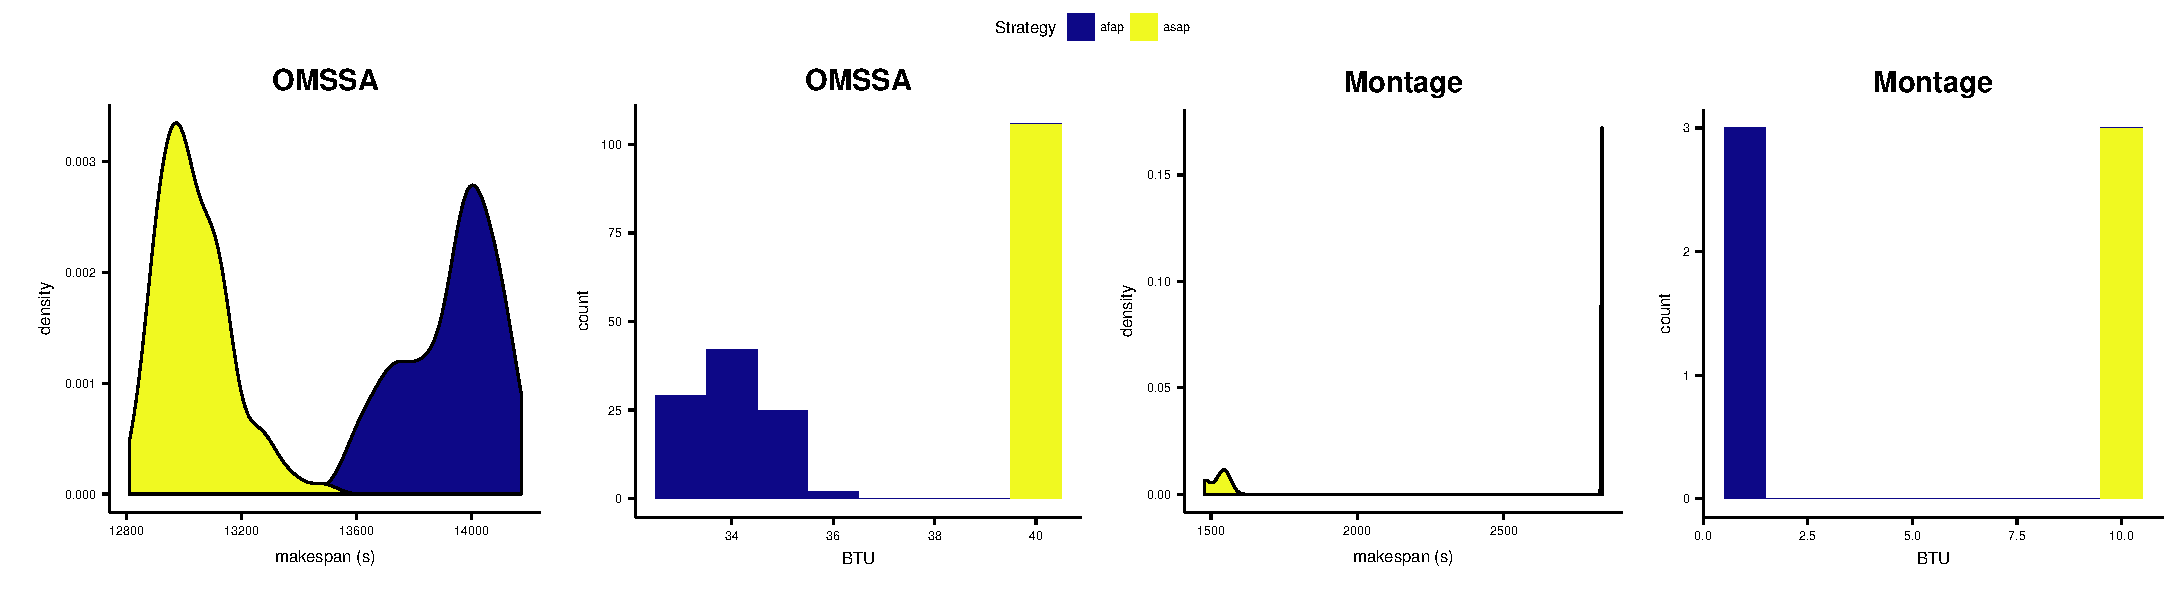
\includegraphics[width=\textwidth]{gfx/real_plot.pdf}
	\caption{Makespan and BTU count distribution for OMSSA and Montage
	runs\label{fig:realbrs}}
\end{figure*}

\subsection{Simulated Execution Setup}
As a follow-up  to our work on Schlouder we  developed SimSchlouder, a simulator
mimicking  the  behaviour  of  Schlouder. Its  implements  the  same  scheduling
strategies  as  Schlouder  using  SimGrid  as its  core  simulation  engine.  In
practice, SimSchlouder  is included as  a plugin  into Schlouder and  allows the
user to request for  an estimate of the makespan and the  cost before choosing a
strategy for a real run.

As  shown on  the right  side of  Figure~\ref{fig:rs}, SimSchlouder  shares with
Schlouder  a common  subset of  inputs.   Its inputs  include the  same job  set
description  and  strategy.    Whereas  Schlouder  operates  on   a  real  cloud
controller,  SimSchlouder   provisions  simulated  \acp{vm}  and   jobs  through
SimGrid's cloud interface  called SchIaaS. As mentioned  earlier, the simulation
requires  additional information  regarding  the  execution platform  simulated,
which is  provided by platform (for  the hardware) and cloud  configuration (for
the cloud resource management  policies) descriptions.  Most importantly, during
a real execution the \emph{effective runtime}  is the real observed runtime of a
job,  which   might  differ  from   the  user  estimate,  used   for  scheduling
purposes. For a better control of the simulation, SimSchlouder can take observed
effective runtimes as inputs.

\begin{comment}
For the purpose of this paper, we classify the inputs required by SimSchlouder
in two categories. The first category is the operator inputs, which describe the
hardware platform and the cloud configuration. Internally, they are fed to the
SimGrid core and the \ac{iaas} simulation layer. The second category is the end
user inputs. They describe the workflow to simulate, the submission dates of
each job, the runtime prediction that would be provided to Schlouder.
Additionally for the purpose of the simulator, a user can choose to supply
effective runtimes to match, communication to simulate, or alternative boot
times for the \acp{vm}. These additional inputs are used to alter the sequence
of events simulated without interfering with parameters that would change the
provisioning or scheduling decisions made by SimSchlouder, e.g.\ having a job
overrun its runtime without changing the corresponding user prediction.

As mentioned above, the variability of real executions suggests that a simulation,
even if it was  perfectly accurate, would capture only one of the set
of possible real executions. We will show later that  the simulation is indeed
very   accurate  when   the  user   estimates  are   close  to   the  effective
runtimes. However,  to  provide the user  with a broader view  of how
their real executions could behave with job runtimes variability,  we should 
enrich the simulation framework with some form of stochastic prediction.
\end{comment}




\begin{comment}
\begin{figure}
	\resizebox{0.5\textwidth}{!}{%
		\usetikzlibrary{fit,arrows}
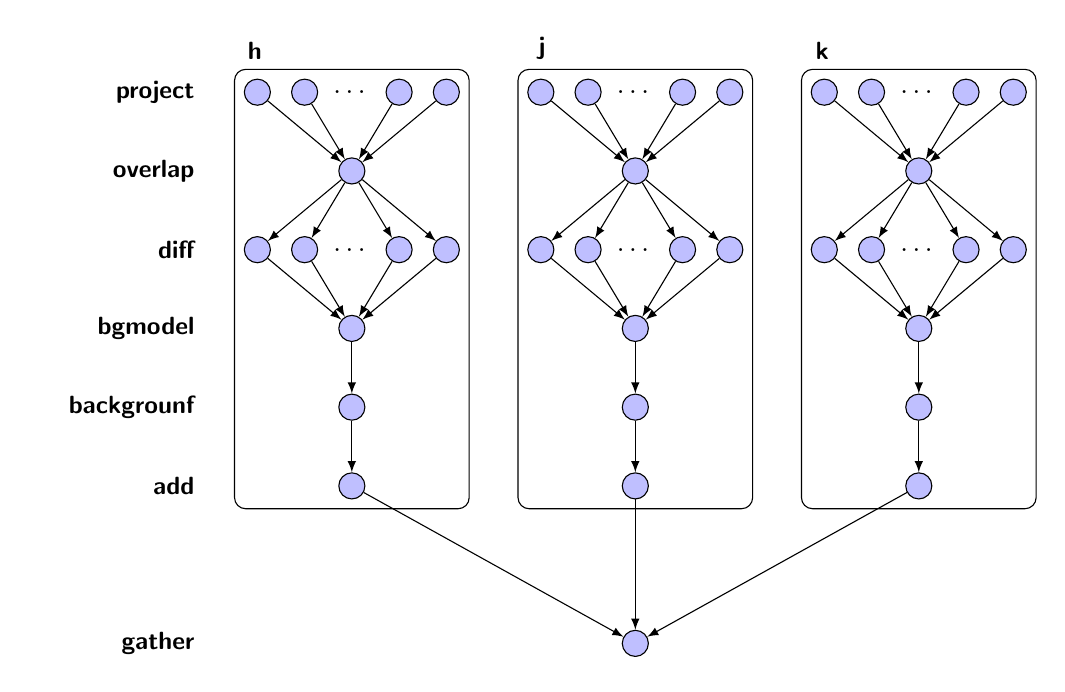
\begin{tikzpicture}[x=6mm,y=-10mm,
task/.style={%
 fill=blue!25,
draw,circle
},
level/.style={%
  font={\sffamily\bfseries\color{black} \fontsize{9pt}{12}\selectfont},
  align=right,
  text width=20mm
},
dot/.style={%
circle
}
]
%levels
\node[level] at (0,0)(Lproj){project};
\node[level] at (0,1)(Loverlap){overlap};
\node[level] at (0,2)(Ldiff){diff};
\node[level] at (0,3)(Lbgm){bgmodel};
\node[level] at (0,4)(Lbg){backgrounf};
\node[level] at (0,5)(Ladd){add};
\node[level] at(0,7)(Lgather){gather};
%%Gather node
\node[task,shift={(9,0)}]at(2,7)(gather){};
%%Loop HJK
\foreach \n [count=\i from 0] in {h,j,k}
{%
\begin{scope}[shift={(3+6*\i,0)}]
% 1 node per group
\node[task]at(2,1)(\i_overlap){};
\node[task]at(2,3)(\i_bgm){};
\node[task]at(2,4)(\i_bg){};
\node[task]at(2,5)(\i_add){};
%% 4 node per group
\foreach \y in {0,1,3,4}
{%
\node[task]at(\y,0)(\i_p_\y){};
\node[task]at(\y,2)(\i_d_\y){};
\draw[-{latex}](\i_p_\y)--(\i_overlap);
\draw[-{latex}](\i_overlap)--(\i_d_\y);
\draw[-{latex}](\i_d_\y)--(\i_bgm);
}
%%4 groups elipsis
\foreach \y in {0,2}
{%
\node[dot]at(2,\y){\ldots};
}
%%single deps
\draw[-{latex}](\i_bgm)--(\i_bg);
\draw[-{latex}](\i_bg)--(\i_add);
%%HJK boxes
\node[rounded corners,draw,fit=(\i_add)(\i_p_0)(\i_p_4),label={[font={\sffamily\bfseries\color{black}\fontsize{9pt}{12}\selectfont}]110:\n}]{};
\end{scope}
%% Gather deps
\draw[-{latex}](\i_add)--(gather);
}
\end{tikzpicture}
		}%
	\caption{Montage workflow diagram.}\label{fig:montage}
\end{figure}

These two applications were executed using Schlouder on a private cloud.  We set
up a 96 core cloud based on four identical  dual $2.67GHz$ Intel Xeon X5650
servers with KVM-based virtualization  and an Openstack cloud-front (first
2012.1, and later 2014.2). This cluster was exclusively used by us and special
attention was taken to never overload the system.



Logs from the executions of these applications display variability in the jobs
individual runtimes, as well as in the application makespan, even when the
execution where scheduled on the same platforms using the same strategies. This
variability is inherent to executions in the cloud. SimSchlouder as shown
promising results when when simulating a given execution, but as a \ac{des} it
is ill-equipped to tackle cases wherein there is uncertainty as to the values of
job runtimes.


\end{comment}

\section{Enriched Simulation Framework}\label{sec:enriched-sim}

\begin{figure}
	\centering
	\resizebox{0.5\textwidth}{!}{%
		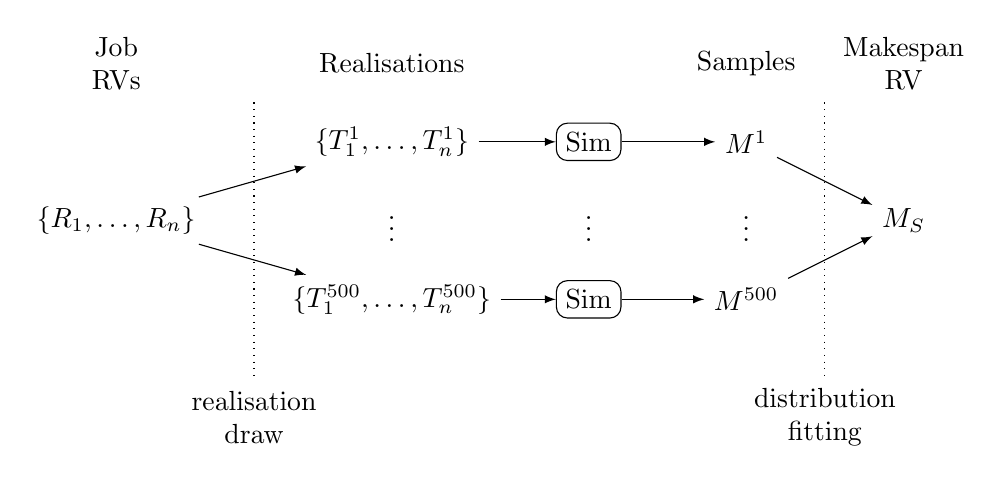
\begin{tikzpicture}[
sim/.style={%
draw, 
rounded corners
}
]
%% Origin node
\node[align=center]at(0,2){Job\\RVs};
\node at(0,0)(orig){$\{R_1,\ldots,R_n\}$};
%% Realisations
\node at(3.5,2){Realisations};
\node[]at(3.5,1)(pert1){$\{T_1^1,\ldots,T_n^1\}$};
\node at(3.5,0){\vdots};
\node at(3.5,-1)(pert5){$\{T_1^{500},\ldots,T_n^{500}\}$};
\draw[-{latex}](orig)--(pert1);
\draw[-{latex}](orig)--(pert5);
%%
\node[sim]at(6,1)(s1){Sim};
\node[sim]at(6,-1)(s5){Sim};
\node at(6,0){\vdots};
\draw[-{latex}](pert1)--(s1);
\draw[-{latex}](pert5)--(s5);
%% Makespans
\node at(8,2){Samples};
\node at(8,1)(M1){$M^1$};
\node at(8,-1)(M5){$M^{500}$};
\node at(8,-0){\vdots};
\draw[-{latex}](s1)--(M1);
\draw[-{latex}](s5)--(M5);
%% Consolidation
\node[align=center]at(10,2){Makespan\\RV};
\node at(10,0)(r){$M_S$};
\draw[-{latex}](M1)--(r);
\draw[-{latex}](M5)--(r);
%%phases
\node[align=center]at(1.75,-2.5)(df){realisation\\draw};
\draw[dotted](1.75,1.5)--(1.75,-2);
\node[align=center]at(9,-2.5)(df){distribution\\fitting};
\draw[dotted](9,1.5)--(9,-2);
\end{tikzpicture}

		}
\caption{Overview of a Monte-Carlo simulation~: $500$ realizations are generated
by drawing runtimes for each of the $n$ jobs provided RVs, every realization is
then simulated, the resulting makespan samples make up the final result.}\label{fig:mc-process}
\end{figure}



As stated in  section~\ref{sc:relwork-stochastic}, trustworthiness of simulation
is questionnable when its result is only one of the many possible outcomes. This
work addresses this issue by  proposing a framework implementing the Monte-Carlo
method  with SimSchlouder  as  simulation engine.   This  solution combines  the
relative  simplicity  of a  \ac{des}  with  the  extensive results  provides  by
stochastic simulations.   This approach guarantees that  our simulation respects
the scheduling and provisioning decisions observed in real life, as the \ac{des}
can easily  be programmed to  reproduce such decisions, whereas  integrating the
implication  of  such  decisions  in  the already  complex  computation  of  the
numerical results of a stochastic would be impossible.

In  this  section we  first  discuss  the  particularities  of the  Monte  Carlo
Simulation applied to our context. Then we present the empirical observations we
used as a reference point for this experiment. At last we will explore the steps
taken to model the input \acp{rv} representing the jobs runtimes.

\subsection{Simulation Process}
\begin{comment}
As  depicted   on  Figure~\ref{fig:mc-process},  we  consider   an  application
consisting of  $n$ jobs, independent  or organized as  a workflow. For  each job
$i  \in\,[1;n]$, we provide  a runtime distribution $T_i$ following the method
described in section~\ref{sec:im}.

One MCS-iteration then consists in 
\end{comment}

The whole extended simulation process,  referred to as \ac{mcs}, applied on an
application consiting of $n$ jobs (as depicted fig.~\ref{fig:mc-process})
consists in applying successive MCS-iterations. Assuming we can provide a
runtime distribution $T_i$ for every job $i$, a MCS-iteration consists in~:
\begin{itemize}
\item making one realization of the runtime  for each job $i$, that is randomly
  drawing a runtime value from the associated $T_i$ to obtain a runtime $t_i$,
\item and once runtimes have been drawn for all jobs, proceed to a simulation
  of the execution with these runtime values to obtain a makespan $m$. 
 This simulation is performed by SimSchlouder.
\end{itemize}
Once we obtain enough makespans $m_k$, we compute  a statistical distribution of
the makespan  as a final \ac{rv} noted $M$.


Because of the \emph{pay-as-you-go} nature of the cloud we extend our simulation
to two output variables: we will not only observe the makespan computed at any
step but also the cost for each execution in number of \ac{btu}, that is the
number of VM-hours started during this simulation.

\begin{comment}
%------------------- le paragraphe précédent remplace le texte suivant utilisé
%------------------- dans HPCC17
The simulation engine SimSchlouder  takes as input the user estimates
$T_1, \ldots , T_n$ for the job runtimes, schedules the jobs and finally outputs
the makespan $M$ of the whole batch.  The user estimates might be inaccurate
and  we describe  hereafter  a method  to characterize  the  impact of  repeated
imprecisions (on each  job runtime) on the final makespan.   We have developed a
\ac{mcs} tool to  compute a confidence interval around the  makespan produced by
simulation.  Let us sketch the overall process (see Fig~\ref{fig:mc-process}):
\begin{itemize} 
\item from  the set of  specified runtimes  $\{T_i\}$, the system  generates $s$
  sets  of perturbed  runtimes $\{T_i^1\},  \ldots, \{T_i^s\}$.   Each perturbed
  runtime  is a  random  value  uniformly drawn  around  $T_i$  (to be explained
  below). We call \emph{realization} each such random draw of a set of perturbed
  runtimes.
\item a simulation  is run for each realization, producing  a makespan $M^i$ and
  BTU count sample for each,
\item a  normal distribution ${\cal  N}(\mu,\sigma)$ is fitted on  the different
  makespan values.
\end{itemize}
% -------------------------------------------------------------------------------

Fitting is done to a normal distribution because, in essence the makespan is the
sum  of the  runtimes of  the jobs  on the  critical path  of the  schedule.  To
measure the impact  of the runtime perturbation on the  makespan, we compute the
range $[\mu-2\sigma;\mu+2\sigma]$ (that is  a 95\% confidence interval) relative
to  the mean  $\mu$. 
\end{comment}

\subsection{Real Observations}

\begin{table} \centering \caption{Overview of archived
	executions}\label{tab:nbruns} 
	\begin{tabular}{llrcc} \toprule
		Application&Strategy&\#runs&BTU count&Makespan ($s$)\\
		\midrule 
		\multirow{2}{*}{OMSSA}&ASAP&106&40&12811 -- 13488\\
				      &AFAP&98&33 -- 36&13564 -- 14172\\ 
		\midrule 
		\multirow{2}{*}{Montage}&ASAP&3&10&1478 -- 1554\\
				        &AFAP&3&1&2833 -- 2837\\
		\bottomrule 
	\end{tabular} 
\end{table}
%% Free floating graphs mus be declared a page in advance
\begin{figure*}
	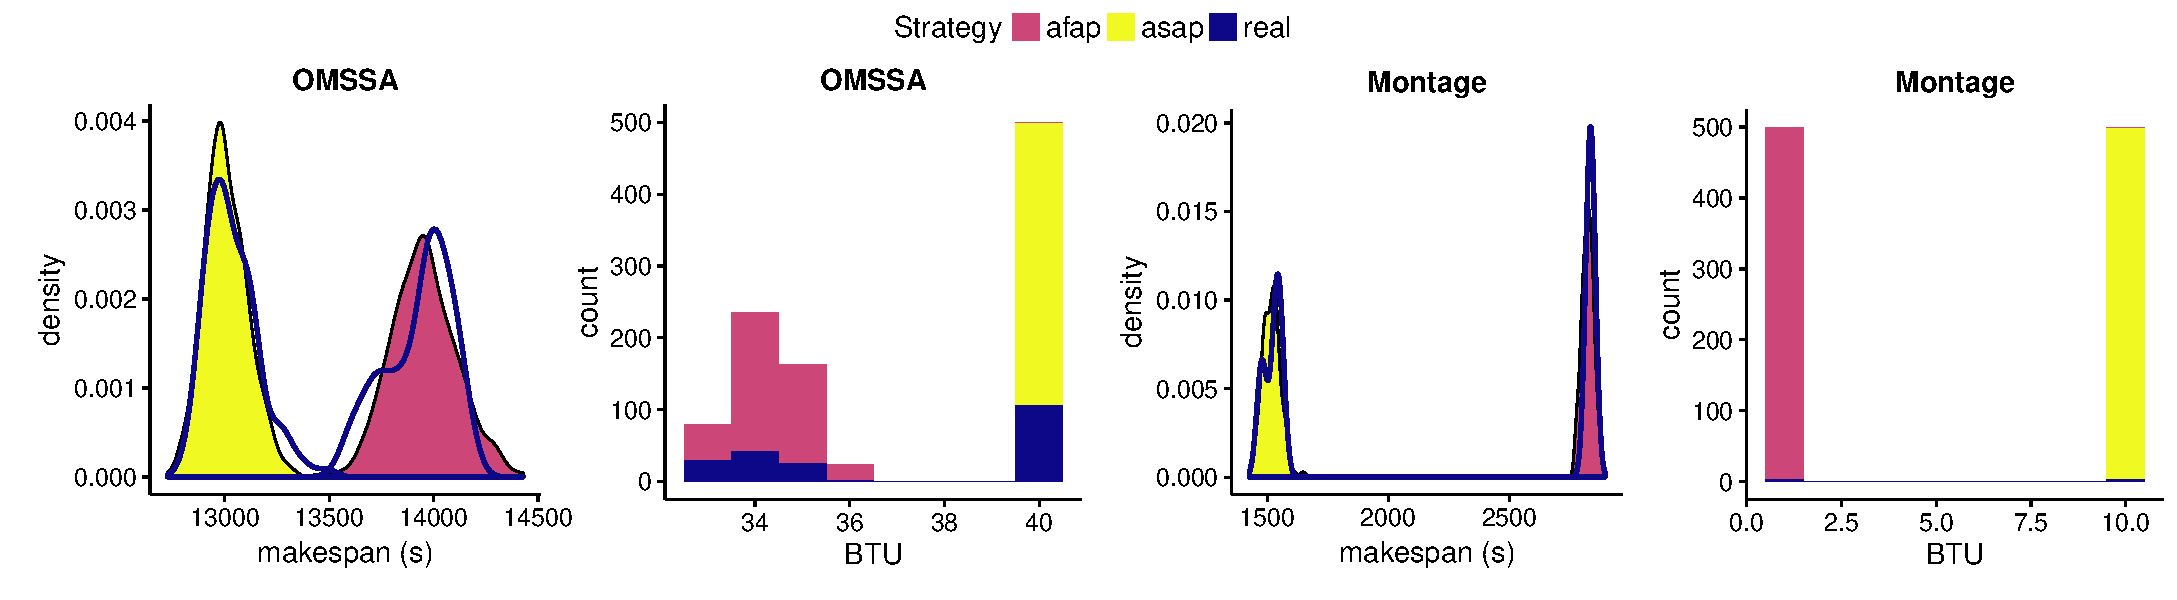
\includegraphics[width=\textwidth]{gfx/fit_plot.pdf}
	\caption{Makespan and BTU count distribution for OMSSA and Montage Monte
	Carlo Simulation compared to reality at 10\% perturbation
	level.}\label{fig:fit}
\end{figure*}


During the development of Schlouder, the cloud broker described in
Section~\ref{sec:work-context}, we performed multiple executions of the
application of OMSSA and Montage. These executions were performed on a 96 core
Openstack cloud system set up on 4 identical dual $2.67GHz$ Intel Xeon X5650
servers. We used the KVM hypervisor and Openstack version 2012.1 and 2014.4.

Schlouder  execution  traces obtained  from  these  experiments contain  several
useful metrics  including, but  not limited  to, the  \ac{vm} start  dates, boot
time, shutdown  times, and assigned  tasks, as well as  the task start  date and
effective  runtimes. We  previously used  these traces  as a  means to  test the
validity of Simschlouder.   These metrics will be used to  generate our \ac{mcs}
input \acp{rv} using the method we will describe in Section~\ref{sec:im}, and we
will compare  the makespan  and \ac{btu}  distributions of  the \ac{mcs}  to the
distribution observed in the corresponding traces.

For this purpose we grouped traces  from comparable runs.  A group contains runs
of a  same application  using the same  strategy on a  same cloud  platform. The
number of observations in  those groups is uneven due to  the changing nature of
the    experimental   conditions    in   which    the   runs    were   executed.
Table~\ref{tab:nbruns}  presents  an  overview   of  the  selected  sets,  while
Figure~\ref{fig:realbrs} presents the distribution of resulting makespans and
\ac{btu} counts observed depending on application and scheduling strategy. These
figures show that even on our platform we observe significant makespan
variability.

\subsection{Input Modeling}\label{sec:im}

The volatile nature  of cloud platform means that effective  runtimes are always
variable. Using a  \ac{mcs} we can account for this  variability and provide the
user with  a range of  possible makespans. In this  section we propose  a simple
method to  represent the variability of  the whole system using  a single factor
parameter to create  a small range around every estimated  runtime. We test this
method against our backlog of real  runs.  The key finding detailed hereafter is
that this simple method  can be precise enough for the  \ac{mcs} to predict over
90\% of real runs.

This model for the runtimes \acp{rv} uses a job's estimated runtime and a global
perturbation  level  for  all  job.   The perturbation  level,  expressed  as  a
percentage an  denoted as  $P$, is used  to build a  range around  the estimated
runtime in which the simulation effective  runtimes will be drawn. If we assume
$P$ can summarize the variability of the whole system, a central question is how
should  be $P$  and the  user estimates  chosen to  assess the  validity of  the
\ac{mcs}.
To that  end, we assume a  good guess for an estimated  runtime is the
average of all effective runtimes for a given job. As such $t_j$, the drawn time
of job $j$, can be written as~:

\begin{equation}
	t_j = \bar{R_j} \cdot (1 + p)
	\label{eq:t}
\end{equation}
\begin{equation}
	\bar{R_j} = \underset{n}{\textrm{mean}}\{r_j^n\}
\end{equation}
\begin{equation}
	p = \mathcal{U}(-P,+P)
	\label{eq:r}
\end{equation}

where $r_j^n$ is the $n$th runtime observation for job $j$, $\bar{R_j}$ is the
average of all observed runtimes for job $j$, and $\mathcal{U}$ an uniform distribution.

To obtain the  global perturbation level $P$, which limits  the worst deviations
from the estimated  runtimes, we average the worst observed  deviation for every
job in the application, formally expressed as :

\begin{equation}
P = \textrm{mean}(\delta{}_j)
\label{eq:P}
\end{equation}
\begin{equation}
\delta{}_j =
\max_n\left(\frac{r_j^n-\bar{R_j}}{\bar{R_j}}\right)
\label{eq:d}
\end{equation}

\begin{comment}
Core  to the  \acl{mcs} is  the accuracy  of our  job runtimes  inputs. Given  a
precise simulator and enough samples, the \ac{mcs} will return a precise result,
but this  result corresponds to  the reality described  by the inputs.  In other
words, for the result to be a good  predictor of the reality, the inputs must be
a good descriptor of reality.

Hence, we seek  to determine which is  the range of acceptable  input values for
the  \ac{mcs} to  produce accurate  enough predictions  (in terms  of confidence
interval),  and we call this  search \emph{input  modeling}.  Answering  this
question will tell us the  acceptable margin of error in the  user estimate for the
method to be relevant.
An ideal  model would present  an individual distribution  for every job  in the
workflow, and such a distribution would require a deep understanding of the jobs
computation, communication, and  of the underlying platform.  In  real life such
modeling  is not  practical  as the  underlying platform  is  usually not
precisely  known, and  the user might not be very familiar with the application.
For this reason, despite having a comprehensive archive ourselves, we choose to 
use a more generic model.

As discussed in Section~\ref{sec:MCS}, for the purpose of our \ac{mcs} we
consider job runtimes as a base runtime on which a perturbation is applied. The
extent of this perturbation is called the \emph{perturbation level} and is
denoted $P$. Though the base is determined job per job, the perturbation level
is set simulation wide. We set the effective runtime of a job $i$ within the
$n$\textit{-th} simulation of an \ac{mcs} to: 
\begin{equation}
	T_i^n = T_i * (1+r_i^n)
\end{equation}
with $r_i^n$ the perturbation value drawn between $[-P;+P]$.

As we  will see  in Section~\ref{sec:sa},  the parameters $T_i$  and $P$  have a
great influence on the \ac{mcs} results.  Our findings are that the best results
are obtained by  taking as $T_i$ the average effective  runtime observed for job
$i$ for a given  strategy. This corresponds to the guess of a knowledgeable user.
Regarding  the simulation  wide perturbation level  $P$, we found  that the best
setting  is the average  of the worst relative deviations for all jobs in the
workload:
\begin{equation}
P = \underset{i}{\textrm{mean}}(\delta{}_i)
\end{equation}
\begin{equation}
\delta{}_i =
\max_n\left(\frac{R_i^n-\textrm{mean}(R_i)}{\textrm{mean}(R_i)}\right)
\end{equation}
with $R_i^n$ the observed effective runtime for job $i$ during execution $n$. 
\end{comment}

For OMSSA, the perturbation level given by this method is $P\approx{}10\%$ for both
strategies. For Montage  our calculated perturbation level is  $P\approx{}20\%$
for ASAP and $P\approx{}5\%$ for AFAP.


\section{Evaluation}
\label{sec:eval}

\begin{table}
	\centering
	\caption{Makespan and BTU capture rate depending on confidence interval
          (CI) for a 10\% perturbation level}\label{tab:fit}
	\begin{tabular}{llccc}
		\toprule
		Application&Strategy&\multicolumn{2}{c}{Makespan (Size of CI)}&BTU\\
                           &         & CI 95\% & CI 99\% &\\
		\midrule
		\multirow{2}{*}{OMSSA}&ASAP&  90\% (3\%)&  98\% (5\%)& 100\%\\
				      &AFAP&  92\% (4\%)& 100\% (6\%)& 100\%\\
		\midrule
		\multirow{2}{*}{Montage}&ASAP& 100\% (2\%)& 100\% (4\%)& 100\%\\
					&AFAP& 100\% (1\%)& 100\% (2\%)& 100\%\\
		\bottomrule
	\end{tabular}
\end{table}

We ran a 500 iteration \ac{mcs} for every strategy-application combination using
the job models described in the previous section. The resulting distributionsare
shown in Figure~\ref{fig:fit}.  The makespan density graphs  show the simulation
result distribution  as filled  curves and the  real observed  executions, taken
from  fig.~\ref{fig:realbrs},  as  non-filled  curves.  On  the  \ac{btu}  count
graphs, for  each tick on  the BTU axis, the  left bar represents  the empirical
data, and  right bar the prediction  from the simulation.  Each  graph shows for
both strategy the distribution of a specific metric for a given application.

When looking at the resulting OMSSA distributions, presented in the two leftmost
graphs,  the distribution  of simulated  makespan range  covers fairly  well the
range of  observed makespans, notwithstanding a  slight right skew and  shift of
the empirical  makespan distribution.  The  OMSSA BTU count  distributions shows
similar results.  The range of BTU  numbers required for an execution is correct
(for  instance, for  AFAP  both empirical  observation  and simulation  indicate
between  33 and  36 BTU  are used)  but the  distributions of  these BTU  counts
slightly differ.


After  this  visual inspection  of  the  results  we  now examine  them  through
statistical confidence intervals.   Since the makespan is in essence  the sum of
the runtimes  of the  jobs in that  executions critical path,  and jobs  are all
distributed  using the  uniform distribution  which  has a  finite variance,  we
consider the Central Limit Theorem applicable.  Fitting to a normal distribution
gives us an average makespan $\mu{}$, and a standard deviation $\sigma{}$. These
can be used to  build \acp{ci}. For the normal distribution  the 95\% \ac{ci} is
defined  as   $[\mu{}-2\sigma{},\mu{}+2\sigma{}]$  and   the  99\%   \ac{ci}  as
$[\mu{}-3\sigma{},\mu{}+3\sigma{}]$.

The capture rate expresses the number of observed real makespans that fall
within a given \ac{ci} relative to the total number of real observations.
Table~\ref{tab:fit} presents the capture rate obtained by each interval computed
after normal fitting.  Additionally we provide for each interval its size
relative to the average makespan.

%%Free floating figure must be declare one page ahead.
\begin{figure*}
	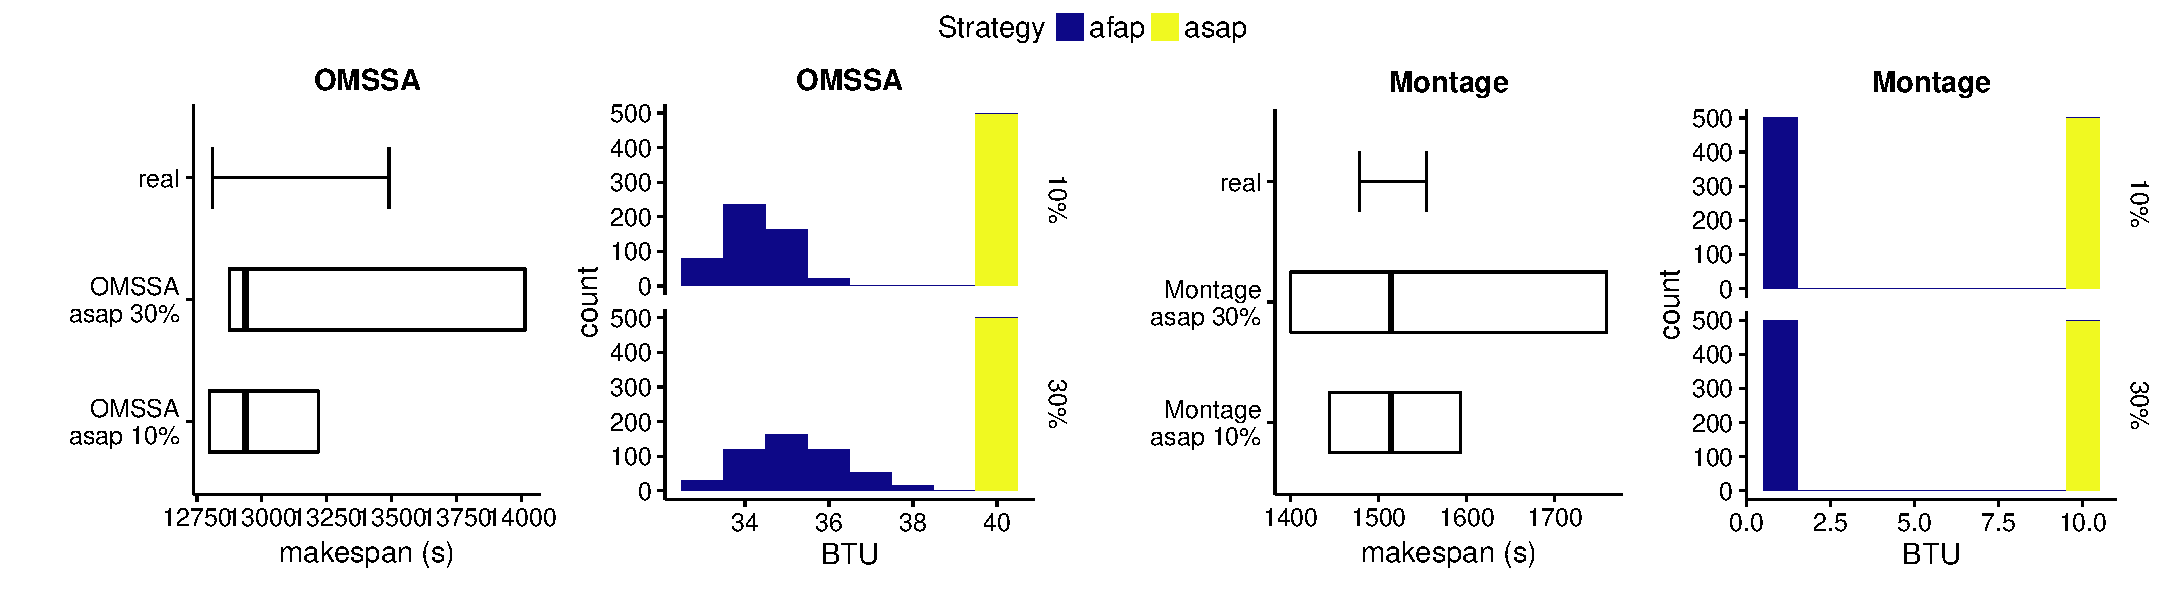
\includegraphics[width=\textwidth]{gfx/int_plot.pdf}
	\caption{Makespan intervals and BTU count distribution for OMSSA and 
	Montage at different perturbation levels. In the makespan interval graph 
	the boxes represent the 95\% \ac{ci} resulting from the normal fit of the
	\acs{mcs}'s results, and the bar the results of a single unperturbed 
	simulation.}\label{fig:int}
\end{figure*}

On OMSSA the  \ac{mcs} captures 90\% of real observed  makespans. The divergence
between the  capture rate and  the \ac{ci} expected capture  rate is due  to the
fact that the  empirical makespan distribution does not follow  a perfect normal
distribution. Using  a 99\% \ac{ci}  improves the capture  rate up to  98\%,
hence very close  the theoretical expectation.   When simulating Montage  the
\ac{mcs} achieves a capture rate of 100\% for any \ac{ci}.

\begin{comment}
The number of Montage runs does not allow to conclusively how well the
simulation matched reality, the obtained results shown in Figure~\ref{fig:fit}
and table~\ref{tab:fit} indicate that Montage's workflow structure does not 
impact the success of the \ac{mcs}.

Simulating Montage with the computed perturbation levels, as discussed in
section~\ref{sec:im} 20\% when using ASAP and 5\% with AFAP, we obtained 100\%
capture rate. The results displayed in Figure~\ref{fig:fit} and
table~\ref{tab:fit} are for simulations done with the 10\% perturbation level.   
Here again the graph shows great coverage. Distribution can not be significantly
tested due to the lackluster number of real runs. The quantitative approach
confirms our observation. The low number of evaluation limits our ability to
have a good look at distribution, but the platform on which these experiments
were run does not exist at this time preventing us from obtaining new real
executions \textbf{FIXME: bien réfléchir si on ne se tire pas une balle dans le
  pied}.
 We kept this limited Montage run as to check that the results
obtained with OMSSA would not completely fail with an application with strong
dependencies. These results give confidence that our method is extendable to
workflow type applications.  
\end{comment}

Our \ac{mcs} and a simple job model can capture 90\% of reality all the while
producing makespan intervals of limited size, a 3\% relative size representing 7
minutes on a 3h 45m long makespan. We consider this result a satisfactory
trade-off between the simplicity of the input model and the accuracy with
regards to the theoretical \ac{ci}.
\begin{comment}
Improving the \ac{mcs} results would require
either more complex inputs models or building ad-hoc \acp{ci} without relying not
the normal distribution.
\end{comment}
Furthermore this \ac{mcs} offers plenty of opportunities other than runtime and
cost predictions.

\begin{comment}
We evaluate the  validity of our simulation based on  two different factors, the
\emph{makespan capture  rate} and  the \emph{BTU capture rate}.   The makespan
capture rate is the percentage of  real makespans which fall into the confidence
interval generated by fitting the  makespans of our individual simulations using
a Normal distribution, as  discussed in Section~\ref{sec:MCS}.  Unless otherwise
specified we  use a standard 95\%  confidence interval of width  $4\sigma$.  BTU
capture rate is the ratio of BTU counts found in the simulation to the BTU
counts observed  during our  real runs.  Figure~\ref{fig:fit} shows  results for
\acp{mcs} using  the input  model presented  in the previous  section at  a 10\%
perturbation level.

Table~\ref{tab:fit}  summarizes the  results obtained  with a  10\% perturbation
level. Along with the makespan capture rates included in parenthesis is the size
of the confidence interval relative to  the average makespan.  With our model we
are able to  capture 90\% of real executions  in ASAP and 92\% of  real AFAP run
for OMSSA\@.  These intervals  span 7  and 10  minutes respectively  whereas the
results in our archive  spread over 10 and 11 minutes.   Using a 99\% confidence
interval results in  better capture rates of  100\% for AFAP and  98\% for ASAP,
but also  in wider intervals  of 15 minutes.  Such  an interval increase  may be
seen as having little impact, like in  our OMSSA use-case exhibiting 3 to 4 hour
runs. Probably this choice of the confidence interval is best left to the user.

For cost prediction our enriched  simulation finds exactly the same possibilities
as experienced in reality, though in  the case of AFAP, repartition favors higher
BTU counts, slightly more than observed in our backlog.

Working on Montage when using \acp{mcs} with the perturbation level of its
respective strategy, as seen in Section~\ref{sec:im}, the capture rate is 100\%
across all strategies. This capture rate is maintained when using the 10\%
perturbation obtained using the OMSSA archive. In this cases the intervals span
from 1.5 to 2.5 minutes for AFAP and ASAP respectively on workflow lasting from
47 and 25 minutes respectively. Because Montage runs in less than 1 hour BTU 
counts are naturally stable, which is perfectly assessed by our simulations.

The results shown in  this section show that provided a  good description of job
runtimes our simulator will provide  good predictions of the possible executions
of these runs. However, though we strived to keep our input modeling as simple
as possible, the  benefits of hindsight provided by the  archive means that only
the users most knowledgeable about their  workload and the targeted platform can
hope to achieve such predictions.  In Section~\ref{sec:lim}, we will discuss the
limits we experienced with this approach. In the next section we show by comparing
different \acp{mcs}  that we are able  to study the behavior  of the strategies
when confronted with different applications and perturbation levels.
\end{comment}




\section{Discussion}
\label{sec:disc}
Outside of the realm of reproduction or predictions, we believe that \ac{mcs}
can have other more research oriented applications. In this section we will
exemplify one such application. Then we will discuss limitation we have
encountered in our work with \ac{mcs}.

\subsection{Strategy Analysis}\label{sec:sa}

We have so  far set the perturbation level  to a value that was  relevant to the
real system observed  (see Section~\ref{sec:im}).  A subsequent  question is how
does   the  prediction   change   when  increasing   this  perturbation   level.
Figure~\ref{fig:int} presents the 95\% \acp{ci} obtained thourgh the normal
distribution fitting of simulations with both a 10\%
and a 40\% perturbation  level. On the makespan interval graphs  (first and third
subfigures  from left  to right)  the boxes  represent the  span of the \ac{ci}
interval. For reference  the vertical bar inside represents  a single simulation
using  the average  runtimes without  any random  element added.   Comparing the
interval of  perturbed simulation  to this unperturbed  simulation allows  us to
better see  the effect of  perturbation on the strategy.   In the middle  row of
these subfigures, are presented for  reference the interval spanning the minimum
and maximum  observed real  makespans over all  runs.  These  \ac{ci} subfigures
only present ASAP strategy whereas  the BTU distribution subfigures present both
strategies.

The leftmost subfigure presents the \acp{ci} for OMSSA using the ASAP strategy at
40\% and 10\% perturbation levels. With the increase of the perturbation level
the intervals naturally get wider, but the average makespan, by definition the
center of the capture interval, also gets higher. On OMSSA this happens to the
extent that the lower bound of our interval at 40\% is higher than the lower
bound at 10\%. This diminishes the capture rate of the simulation from 90\%
(table~\ref{tab:fit}) to 83\% even as the relative width of the interval grows
from 3\% (7 minutes) to 10\% (almost 24 minutes).

This result is two-fold. First this demonstrates that the perturbation level can
not be used as a trade-off variable to augment capture rate at the expense of
\ac{ci} compacity. The lower capture rate at a 40\% perturbation level is a
strong indication that our real platform exhibits a variability closer to
10\% than to 40\%. People for whom higher capture rates are more important than
interval compacity should use statistical methods to build higher rate \acp{ci},
like the 99\% normal distribution \ac{ci} use in section~\ref{sec:eval}.

Secondly this result shows how an \ac{mcs} can be used to exhibit strategy
behaviours. This upwards shift of the \ac{ci} shows that ASAP, a strategy
geared towards reducing the makespan regardless of cost, is not as effective
when scheduling bag-of-tasks in environments where job runtimes might vary
widely. By testing Montage in the same way (third subfigure) we see that when
scheduling workflows this behaviour does not happen to the same extent. The
average makespan still rises, but not as fast as the interval grows, the \ac{ci}
at a 40\% perturbation level is a superset of the one at a 10\% perturbation
level. In the case of ASAP we can explain this behaviour is explained by the
fact that when using ASAP the last job of every \ac{vm} are synchronized,
therefore any runtime exceeding it's expected value will extend the makespan.
But this kind of analysis can be used to gain insight in the strengths and
weaknesses of complex strategies.


\subsection{Advantages and limitations of the enriched simulation}\label{sec:lim}

In this section we discuss parameters that one might want to account for when
using an \ac{mcs}. At these points in time we have not yet studied how they
influence the \ac{mcs} or its result but are looking on to evaluate them in
future works.

In this article the only variable parameter is jobs runtimes. As such these
runtimes coalesce all sources of variability, change in available CPU time,
network or memory contention and application inherent variability. We did so
because this approach is closer to a cloud broker user scenario and  the
execution traces we had did not allow for us to separate in a convincing way these
different variability sources. In circumstance where one is able to measure variability
on CPU power or network speed it is possible to add those variable as input of
the \ac{mcs}. In this case a realization would draw not only each jobs size 
 but also a platform with different CPU powers and network speed.
\ac{mcs} enables to fuse these different variability sources effortlessly, but it will
require more iterations. 

In this paper all the \ac{mcs} presented used 500 iterations, that is 500
different runs of our \ac{des}. We determined that this was enough in the
context of our simulation as additional simulation did not change the results
and only marginally increased the confidence of the fitting process. The number
of simulation necessary in an \ac{mcs} depends on the number of input variables
and the distribution of these variables. \aclp{mcs} work by sampling the possible
scenarios to get a distribution of possible. As such the more scenarios are
possible the more samples are required. In our cases not only the number of jobs
was low, 223 jobs for OMSSA and 184 jobs for Montage, but with a 10\%
perturbation level the input variable distribution was compact. At a 40\%
perturbation level there was a significant drop in the confidence of our fitting
method. We are currently studying the relationship between perturbation level
and the number of required MCS-iterations.

\section{Conclusion}
Predicting  the execution  behavior  of complex  workloads in  the  cloud is  an
important challenge. While a number of research works have proposed model-driven
simulators, much remains to be done for their adoption in production-grade cloud
settings. As  advocated by Puchert  et al.~\cite{PucherGWK15}, the trust  we can
put in  the prediction  demands certainty  and precision  that only  comes from
validating simulation against empirical observation.

This paper contributes to this effort in two ways. First, we propose a \acl{mcs}
extension  to a  discrete  event  simulator based  on  SimGrid.  This  extension
provides stochastic predictions which are more informative than single values of
rental cost  and makespan  produced by  traditionnal discrete  event simulators.
The \acl{mcs}  must be parameterized to  draw random values from  relevant value
spaces. In this work we show that the  variability we seek to account for can be
modeled  by a  single parameter  called perturbation  level applied  to all  job
runtimes. Second, we apply our method in  a real setting, on both a bag-of-tasks
and a workflow application for which we have collected execution traces.  Thanks
to these empirical observations, our study  shows that the proposed method could
capture over  90\% of the  observed makespans given an  appropriate perturbation
level.

The  first  perspective of  this  work  is to  apply  the  method to  production
clouds.  In this  paper we  managed to  aggregate all  the different  sources of
uncertainty  into a  perturbation on  the job's  runtime. We  are interested  in
checking whether  this is  still possible in  highly variable  environments. Our
second  perspective, now  that  we  are confident  in  our  ability to  simulate
application executions, is to move away from the applications in our archive and
use our  enriched simulation  to study the  interactions between  scheduling and
workflow.  More specifically,  we  are  interested in  how  the  structure of  a
workflow  affects a  scheduling's robustness,  that is,  its ability  to satisfy
predetermined  in terms of deadline or cost.





\bibliographystyle{IEEEtran}
\bibliography{montecarlo-simulation}



\newpage

\end{document}
% vim:spell spelllang=en:
